\documentclass[12pt,addpoints]{evalua}
\grado{2$^\circ$ de Secundaria}
\cicloescolar{2023-2024}
\materia{Matemáticas 2}
\unidad{1}
\title{Examen de la Unidad}
\aprendizajes{
        \item Resuelve problemas de multiplicación y división con números enteros, fracciones y decimales positivos y negativos.
        \item Resuelve problemas de potencias con exponente entero y aproxima raíces cuadradas.
        \item Resuelve problemas de proporcionalidad directa e inversa y de reparto proporcional.
}
\author{Prof.: Julio César Melchor Pinto}
\begin{document}
\begin{questions}
      \question[10] Escribe sobre la línea el símbolo de mayor que ($>$), menor que ($<$), o igual ($=$) según corresponda.

      \begin{multicols}{2}
            \begin{parts}
                  % \part $\dfrac{2}{5}$ \fillin[$>$][0.5in] $\dfrac{1}{3}$\\[0.75em]
                  % \part $\dfrac{3}{4}$ \fillin[$<$][0.5in] $\dfrac{4}{5}$\\[0.75em]
                  % \part $\dfrac{2}{5}$ \fillin[$<$][0.5in] $\dfrac{2}{3}$\\[0.75em]
                  % \part $\dfrac{3}{2}$ \fillin[$=$][0.5in] $\dfrac{9}{6}$\\[0.75em]
                  % \part $\dfrac{5}{6}$ \fillin[$>$][0.5in] $\dfrac{4}{6}$\\[0.75em]
                  % \part $\dfrac{4}{3}$ \fillin[$>$][0.5in] $\dfrac{5}{4}$\\[0.75em]
                  % \part $\dfrac{1}{3}$ \fillin[$=$][0.5in] $\dfrac{9}{3}$\\[0.75em]
                  % \part $\dfrac{2}{3}$ \fillin[$<$][0.5in] $\dfrac{3}{2}$\\[0.75em]
                  % \part $\dfrac{3}{4}$ \fillin[$>$][0.5in] $\dfrac{2}{3}$\\[0.75em]
                  % \part $\dfrac{5}{6}$ \fillin[$>$][0.5in] $\dfrac{4}{5}$\\[0.75em]
                  \part $-51$ \fillin[$>$][0.5in] $-55$\\[0.75em]
                  \part $-77$ \fillin[$>$][0.5in] $-177$\\[0.75em]
                  \part $-100$ \fillin[$<$][0.5in] $-99$\\[0.75em]
                  \part $-182$ \fillin[$>$][0.5in] $-189$\\[0.75em]
                  \part $-97$ \fillin[$<$][0.5in] $-96.2$\\[0.75em]
                  \part $-36$ \fillin[$>$][0.5in] $-39$\\[0.75em]
                  \part $-3.5$ \fillin[$<$][0.5in] $-2.2$\\[0.75em]
                  \part $-12$ \fillin[$<$][0.5in] $-11$\\[0.75em]
                  \part $-10.001$ \fillin[$>$][0.5in] $-100.01$\\[0.75em]
                  \part $-0.99$ \fillin[$>$][0.5in] $1.01$\\[0.75em]
            \end{parts}
      \end{multicols}

      \question[15] Convierte los siguientes números en notación decimal a notación científica en la forma más reducida posible.
      \begin{multicols}{2}
            \begin{parts}
                  % \part $50500=$ \fillin[$5.05 \cdot 10^4$][1.5in]
                  % \part $0.00000000024=$ \fillin[$2.4 \cdot 10^{-10}$][1.5in]
                  % \part $101=$ \fillin[$1.01 \cdot 10^2$][1.5in]
                  % \part $750000000000=$ \fillin[$7.5 \cdot 10^{11}$][1.5in]
                  \part $80008000=$ \fillin[$8.0008 \cdot 10^7$][1.5in]
                  \part $0.003=$ \fillin[$3 \cdot 10^{-3}$][1.5in]
                  \part $0.0000204=$ \fillin[$2.04 \cdot 10^{-5}$][1.5in]
                  \part $0.0000000000099=$ \fillin[$9.9 \cdot 10^{-12}$][1.5in]
                  % \part $606000000000000000=$ \fillin[$6.06 \cdot 10^{17}$][1.5in]
                  \part $102100000000000=$ \fillin[$1.001 \cdot 10^{-7}$][1.5in]
            \end{parts}
      \end{multicols}

      \newpage

      \question[20] Realiza las operaciones con exponentes indicadas en cada uno de los siguientes incisos.

      \begin{multicols}{2}
            \begin{parts}
                  \part $x^2y^3z^4 \cdot x^5z^4=$
                  \begin{solutionbox}{2cm}
                        $x^2y^3z^4 \cdot x^5z^4 = x^7y^3z^8$
                  \end{solutionbox}

                  % \part $x^3x^2x^3=$
                  % \begin{solutionbox}{2cm}
                  %       $x^3x^2x^3 = x^8$
                  % \end{solutionbox}

                  \part $7x^2\cdot 3x^4 \cdot 6x^2=$
                  \begin{solutionbox}{2cm}
                        $7x^2\cdot 3x^4 \cdot 6x^2 = 126x^8$
                  \end{solutionbox}

                  % \part $(-4x^2)(-5x^3)=$
                  % \begin{solutionbox}{2cm}
                  %       $(-4x^2)(-5x^3) = 20x^5$
                  % \end{solutionbox}

                  % \part $(-8x)(-5x^5)=$
                  % \begin{solutionbox}{2cm}
                  %       $(-8x)(-5x^5) = 40x^6$
                  % \end{solutionbox}

                  \part $(-x^4)(2y^3)=$
                  \begin{solutionbox}{2cm}
                        $(-x^4)(2y^3) = -2x^4y^3$
                  \end{solutionbox}

                  % \part $(-5a^4)(-3a^2)=$
                  % \begin{solutionbox}{2cm}
                  %       $(-5a^4)(-3a^2) = 15a^6$
                  % \end{solutionbox}

                  \part  $x^3\cdot x^5\cdot x=$
                  \begin{solutionbox}{2cm}
                        $x^3\cdot x^5\cdot x = x^9$
                  \end{solutionbox}

                  % \part $(-3a^4)(8a^2)=$
                  % \begin{solutionbox}{2cm}
                  %       $(-3a^4)(8a^2) = -24a^6$
                  % \end{solutionbox}

                  \part $4x^2\cdot x^5\cdot 5x^8=$
                  \begin{solutionbox}{2cm}
                        $4x^2\cdot x^5\cdot 5x^8 = 20x^{15}$
                  \end{solutionbox}

                  \part $\dfrac{x^{13}y^{18}z^4}{x^{11}y^9z^4}=$
                  \begin{solutionbox}{2cm}
                        $\dfrac{x^{13}y^{18}z^4}{x^{11}y^9z^4} = x^2y^9$
                  \end{solutionbox}

                  \part $\dfrac{81a^5b^{12}c^9}{9a^3b^{7}c^5}=$
                  \begin{solutionbox}{2cm}
                        $\dfrac{81a^5b^{12}c^9}{9a^3b^{7}c^5} = 9a^2b^5c^4$
                  \end{solutionbox}

                  \part $\dfrac{x^{4}y^{12}z^{13}}{x^{3}y^{12}z^{13}}=$
                  \begin{solutionbox}{2cm}
                        $\dfrac{x^{4}y^{12}z^{13}}{x^{3}y^{12}z^{13}} = x$
                  \end{solutionbox}

                  % \part $\left(a^3 b^5 c^{11} \right)^7=$
                  % \begin{solutionbox}{2cm}
                  %       $\left(a^3 b^5 c^{11} \right)^7 = a^{21}b^{35}c^{77}$
                  % \end{solutionbox}

                  \part $\left(x^4 y^5\right)^6=$
                  \begin{solutionbox}{2cm}
                        $\left(x^4 y^5\right)^6 = x^{24}y^{30}$
                  \end{solutionbox}

                  \part $\left(a^4b^4c^5d^{11}\right)^9=$
                  \begin{solutionbox}{2cm}
                        $\left(a^4b^4c^5d^{11}\right)^9 = a^{36}b^{36}c^{45}d^{99}$
                  \end{solutionbox}
            \end{parts}
      \end{multicols}

      \newpage
      \question[15] Realiza las siguientes operaciones.
      \begin{multicols}{2}
            \begin{parts}
                  \part $2381 \divisionsymbol 1000=$ \fillin[$2.381$][0.5in] \\[1em]
                  % \part $32 \times 100=$ \fillin[$3200$][0.5in] \\[1em]
                  % \part $3461 \divisionsymbol 1000=$ \fillin[$3.461$][0.5in] \\[1em]
                  \part $0.09 \times 100=$ \fillin[$9$][0.5in] \\[1em]
                  \part $\dfrac{3}{10}+\dfrac{4}{5}=$ \fillin[$\dfrac{11}{10}$ o 1$\dfrac{1}{10}$][0.5in] \\[1em]
                  % \part $\dfrac{3}{4}-\dfrac{2}{5}=$ \fillin[$\dfrac{7}{20}$][0.5in] \\[1em]
                  \part $\dfrac{2}{3}-\dfrac{2}{5}=$ \fillin[$\dfrac{4}{15}$][0.5in] \\[1em]
                  % \part $\dfrac{3}{8}+\dfrac{7}{10}=$ \fillin[$\dfrac{43}{40}$ o 1$\dfrac{3}{40}$][0.5in] \\[1em]
                  % \part $\dfrac{7}{10}+\dfrac{2}{5}=$ \fillin[$\dfrac{11}{10}$ o 1$\dfrac{1}{10}$][0.5in] \\[1em]
                  % \part $\dfrac{3}{4}-\dfrac{2}{5}=$ \fillin[$\dfrac{7}{20}$][0.5in] \\[1em]  
                  \part $3\dfrac{1}{2}-1\dfrac{1}{3}$ \fillin[$2\dfrac{1}{6}$][0.5in] \\[1em]
                  % \part $2\frac{2}{3}-2\frac{2}{5}$ \fillin[$\dfrac{4}{15}$][0.5in] \\[1em]
            \end{parts}
      \end{multicols}

      \question[10] Escribe el número que representa el punto indicado en la recta numérica de cada uno de los siguientes incisos.
      \begin{multicols}{2}
            \begin{parts}
                  \part 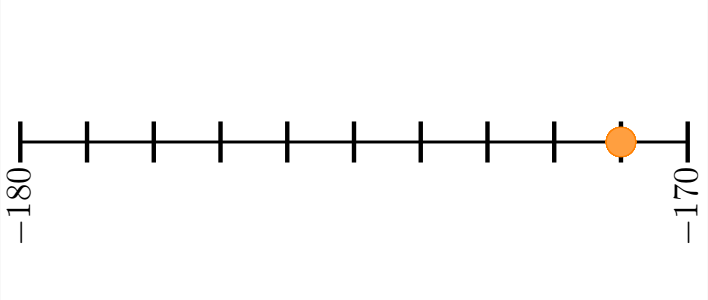
\includegraphics[width=140px]{../images/recta_num_-171.png} \\[-0.5em]   \fillin[$-171$][1.5in]
                  \part 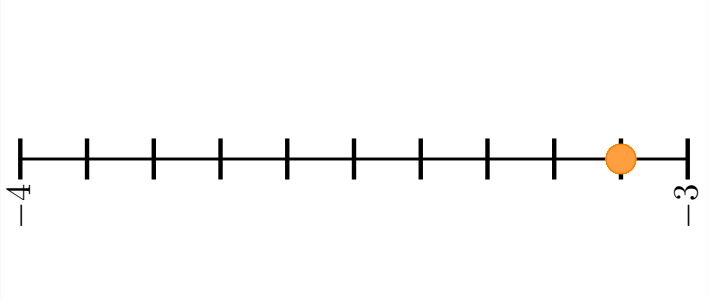
\includegraphics[width=140px]{../images/recta_num_-3.1.png} \\[-0.5em]   \fillin[$-3.1$][1.5in]
                  \part 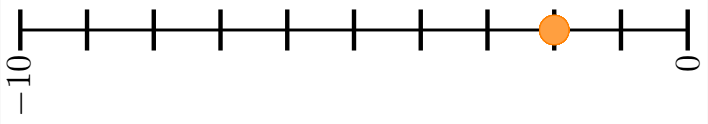
\includegraphics[width=140px]{../images/recta_num_-2.png}   \\[-0.5em] \fillin[$-2$][1.5in]
                  \part 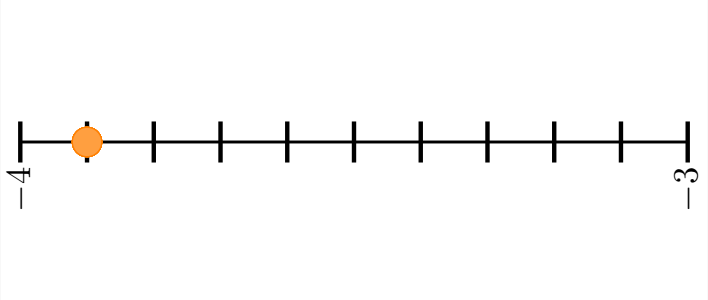
\includegraphics[width=140px]{../images/recta_num_-3.9.png} \\[-0.5em]   \fillin[$-3.9$][1.5in]
                  \part 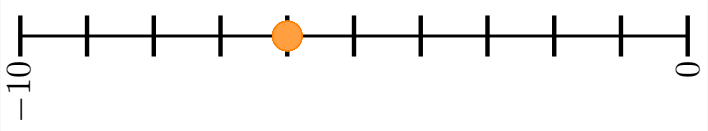
\includegraphics[width=140px]{../images/recta_num_-6.png}   \\[-0.5em] \fillin[$-6$][1.5in]
                  % \part 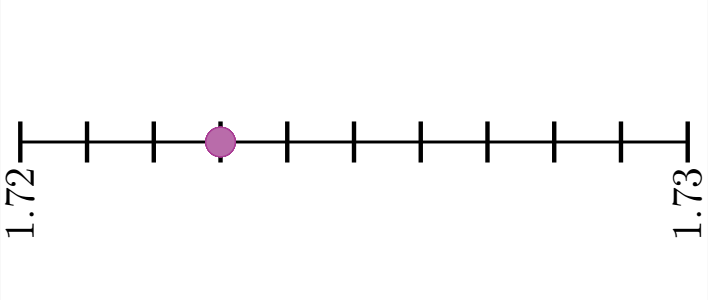
\includegraphics[width=140px]{../images/recta_num_1.723.png}\\[-0.5em]  \fillin[$1.723$][1.5in]
                  % \part 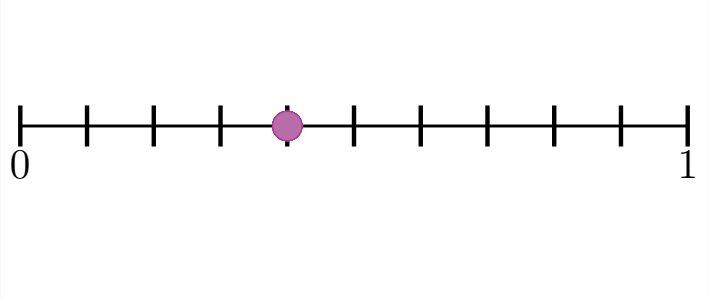
\includegraphics[width=140px]{../images/recta_num_0.4.png}  \\[-0.5em]  \fillin[$0.4.$][1.5in]
                  % \part 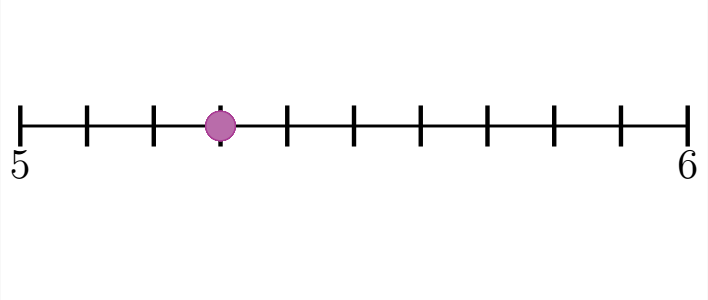
\includegraphics[width=140px]{../images/recta_num_5.3.png}  \\[-0.5em]  \fillin[$5.3.$][1.5in]
                  % \part 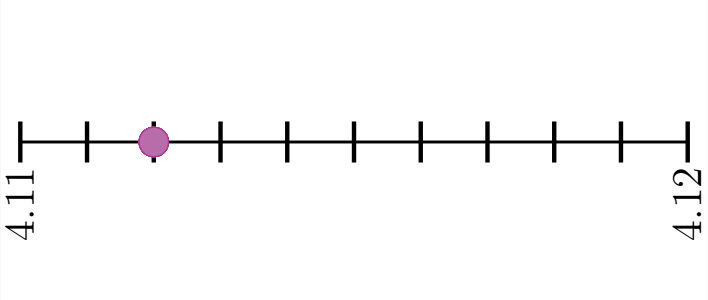
\includegraphics[width=140px]{../images/recta_num_4.112.png}\\[-0.5em]  \fillin[$4.11$][1.5in]
                  % \part 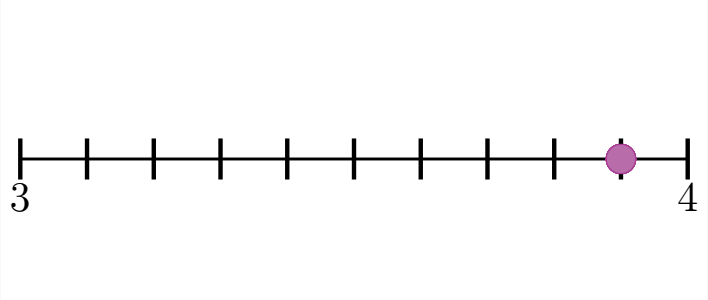
\includegraphics[width=140px]{../images/recta_num_3.9.png}  \\[-0.5em]  \fillin[$3.9.$][1.5in]
                  % \part 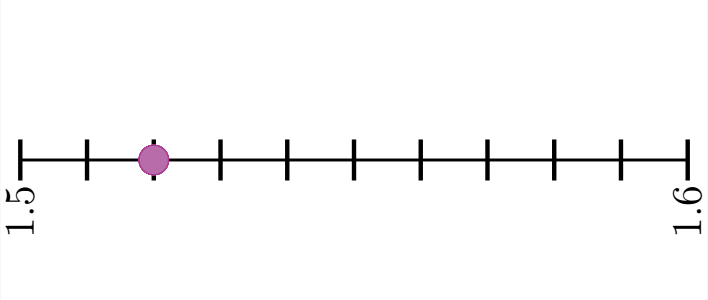
\includegraphics[width=150px]{../images/recta_num_1.52.png} \\[-0.5em] \fillin[$1.52$][1.5in]   \\[-1.4em]
                  \part 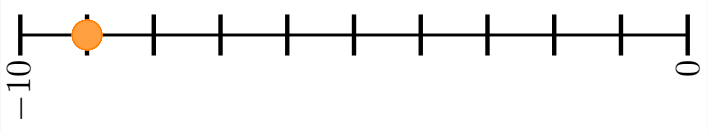
\includegraphics[width=150px]{../images/recta_num_-9.png}   \\[-0.5em] \fillin[$-9$][1.5in]     \\[-1.4em]
                  \part 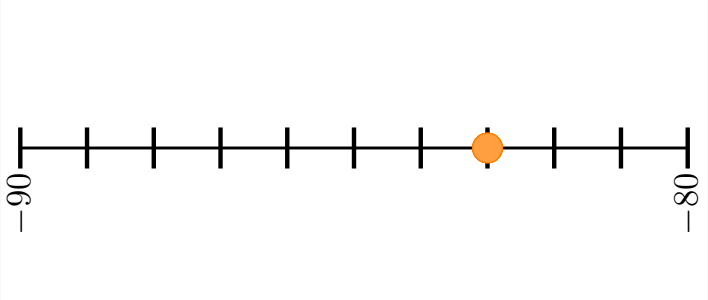
\includegraphics[width=150px]{../images/recta_num_-83.png}  \\[-0.5em]  \fillin[$-83$][1.5in]   \\[-1.4em]
                  % \part 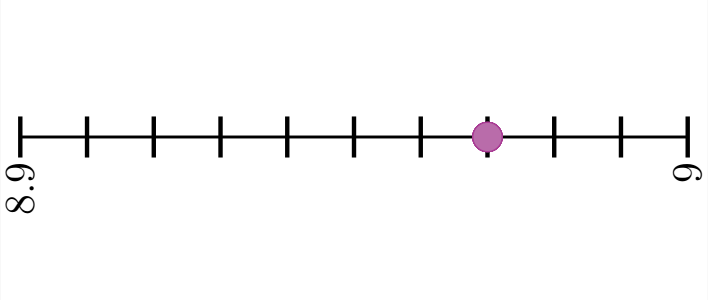
\includegraphics[width=150px]{../images/recta_num_8.97.png} \\[-0.5em]  \fillin[$8.97$][1.5in]  \\[-1.4em]
                  \part 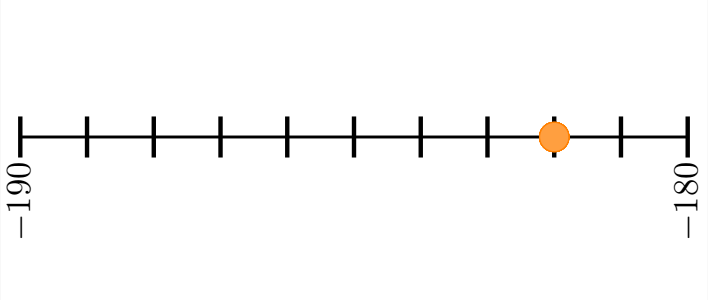
\includegraphics[width=150px]{../images/recta_num_-182.png} \\[-0.5em]   \fillin[$-182$][1.5in] \\[-1.4em]
                  % \part 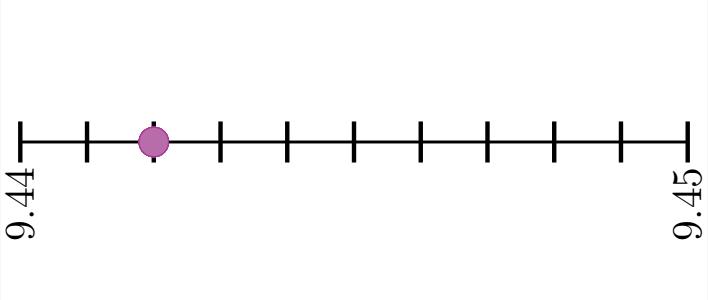
\includegraphics[width=150px]{../images/recta_num_9.442.png}\\[-0.5em]  \fillin[$9.44$][1.5in]  \\[-1.4em]
                  \part 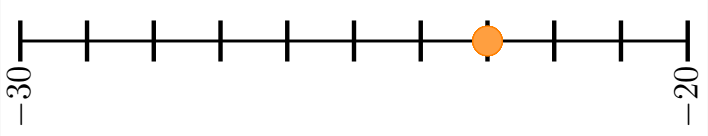
\includegraphics[width=150px]{../images/recta_num_-23.png}  \\[-0.5em]  \fillin[$-23$][1.5in]   \\[-1.4em]
                  % \part 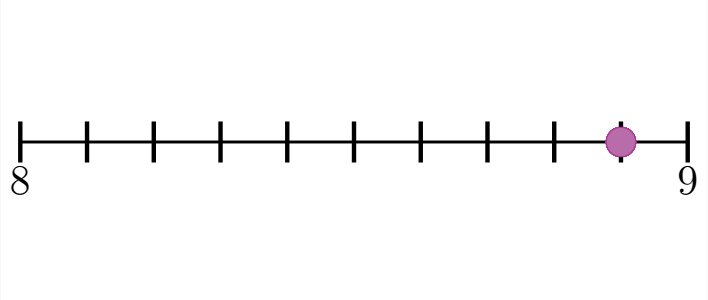
\includegraphics[width=150px]{../images/recta_num_8.9.png}  \\[-0.5em]  \fillin[$8.9$][1.5in]   \\[-1.4em]
                  % \part 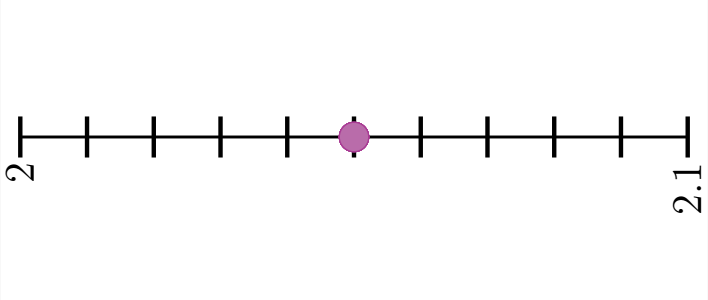
\includegraphics[width=150px]{../images/recta_num_2.05.png} \\[-0.5em]  \fillin[$2.05$][1.5in]  \\[-1.4em]
                  \part 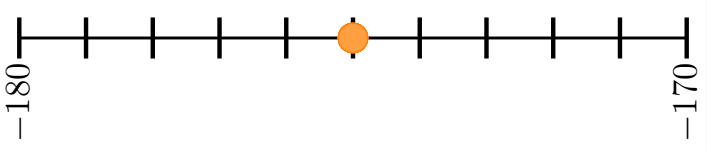
\includegraphics[width=150px]{../images/recta_num_-175.png} \\[-0.5em]   \fillin[$-175$][1.5in]
            \end{parts}
      \end{multicols}

      \newpage
      \question[10] Contesta la pregunta en cada uno de los siguientes problemas.
      \begin{multicols}{2}
            \begin{parts}
                  \part Un carpintero quiere cortar una plancha de madera de 252 cm de largo y 180 cm de ancho, en cuadrados lo más grandes posible. \textbf{¿Cuál debe ser la longitud del lado de cada cuadrado?}
                  \begin{solutionbox}{3.5cm}\scriptsize
                        El tamaño de los cuadrados que debe cortar se calcula con el máximo común divisor de 252 y 180, ya que es la cantidad más grande en que se puede dividir cada uno de los números sin que sobre ninguna madera.
                        \begin{align*}
                              \text{MCD}(252,180) & = 36
                        \end{align*}
                        Por lo tanto, debe cortar cuadrados de 36 cm de lado.
                  \end{solutionbox}

                  \part Una computadora tiene un disco duro de 368 GB de memoria, si varios programas ocupan 128.75 GB. \textbf{¿Qué cantidad de memoria está libre?}
                  \begin{solutionbox}{3cm}\scriptsize
                        La cantidad de memoria libre se calcula restando la memoria que ocupan los programas a la memoria total.
                        \begin{align*}
                              368 - 128.75 & = 239.25
                        \end{align*}
                        Por lo tanto, la cantidad de memoria libre es de 239.25 GB.
                  \end{solutionbox}

                  \part Una pintura tiene un costo de 25.75 pesos el litro, una persona compra 48 litros. \textbf{¿Cuánto debe pagar?}
                  \begin{solutionbox}{3cm}\scriptsize
                        El precio que debe pagar se calcula multiplicando el precio por litro por el número de litros.
                        \begin{align*}
                              25.75 \times 48 & = 1236
                        \end{align*}
                        Por lo tanto, debe pagar 1236 pesos.
                  \end{solutionbox}

                  \part Luis pagó 94.50 pesos en una sala de videojuegos, en donde por esa cantidad le dieron 21 fichas para jugar. \textbf{¿Cuál es el precio que pagó por una ficha?}
                  \begin{solutionbox}{3.5cm}\scriptsize
                        El precio que pagó por una ficha se calcula dividiendo el precio total entre el número de fichas.
                        \begin{align*}
                              \dfrac{94.50}{21} & = 4.5
                        \end{align*}
                        Por lo tanto, el precio que pagó por una ficha es de 4.5 pesos.
                  \end{solutionbox}

                  \part La mamá de Susana compró 11 metros de franela y pagó 103.40 pesos. \textbf{¿Cuánto cuesta el metro de franela?}
                  \begin{solutionbox}{2.5cm}\scriptsize
                        El precio del metro de franela se calcula dividiendo el precio total entre el número de metros.
                        \begin{align*}
                              \dfrac{103.40}{11} & = 9.4
                        \end{align*}
                        Por lo tanto, el precio del metro de franela es de 9.4 pesos.
                  \end{solutionbox}

                  \part El precio de 385 artículos comerciales es de 1,232 pesos. \textbf{¿Cuál es el precio unitario de cada artículo?}
                  \begin{solutionbox}{3.5cm}\scriptsize
                        El precio unitario de cada artículo se calcula dividiendo el precio total entre el número de artículos.
                        \begin{align*}
                              \dfrac{1232}{385} & = 3.2
                        \end{align*}
                        Por lo tanto, el precio unitario de cada artículo es de 3.2 pesos.
                  \end{solutionbox}
            \end{parts}
      \end{multicols}

      \newpage
      \question[10] Identifica la pendiente y ordenada de las rectas en los siguientes incisos.
      \begin{multicols}{2}
            \begin{parts}
                  \part $y=-x$\\[0.5em]
                  Pendiente: \fillin[$-1$][0.5in] Ordenada: \fillin[$0$][0.5in]\\[1em]
                  \part $y=2x$\\[0.5em]
                  Pendiente: \fillin[$2$][0.5in] Ordenada: \fillin[$0$][0.5in] \\[1em]
                  \part $y=3x+7$\\[0.5em]
                  Pendiente: \fillin[$3$][0.5in] Ordenada: \fillin[$7$][0.5in] \\[1em]
                  \part $y=-2x+1$\\[0.5em]
                  Pendiente: \fillin[$-2$][0.5in] Ordenada: \fillin[$1$][0.5in] \\[1em]
                  \part $y=7x+7$\\[0.5em]
                  Pendiente: \fillin[$7$][0.5in] Ordenada: \fillin[$7$][0.5in] \\[1em]
                  \part $y=-\dfrac{1}{2}x-2$\\[0.5em]
                  Pendiente: \fillin[$-\dfrac{1}{2}$][0.5in] Ordenada: \fillin[$-2$][0.5in] \\[1em]
                  \part $y=\dfrac{2}{3}x+5$\\[0.5em]
                  Pendiente: \fillin[$\dfrac{2}{3}$][0.5in] Ordenada: \fillin[$5$][0.5in] \\[1em]
                  \part $y=-5x-4$\\[0.5em]
                  Pendiente: \fillin[$-5$][0.5in] Ordenada: \fillin[$-4$][0.5in] \\[1em]
                  \part $y=-x-1$\\[0.5em]
                  Pendiente: \fillin[$-1$][0.5in] Ordenada: \fillin[$-1$][0.5in] \\[1em]
                  \part $y=-2$\\[0.5em]
                  Pendiente: \fillin[$0$][0.5in] Ordenada: \fillin[$-2$][0.5in] \\[1em]
            \end{parts}
      \end{multicols}

      \question[10] Escribe el número que representa el punto indicado en la recta numérica de cada uno de los siguientes incisos.
      \begin{multicols}{2}
            \begin{parts}
                  \part 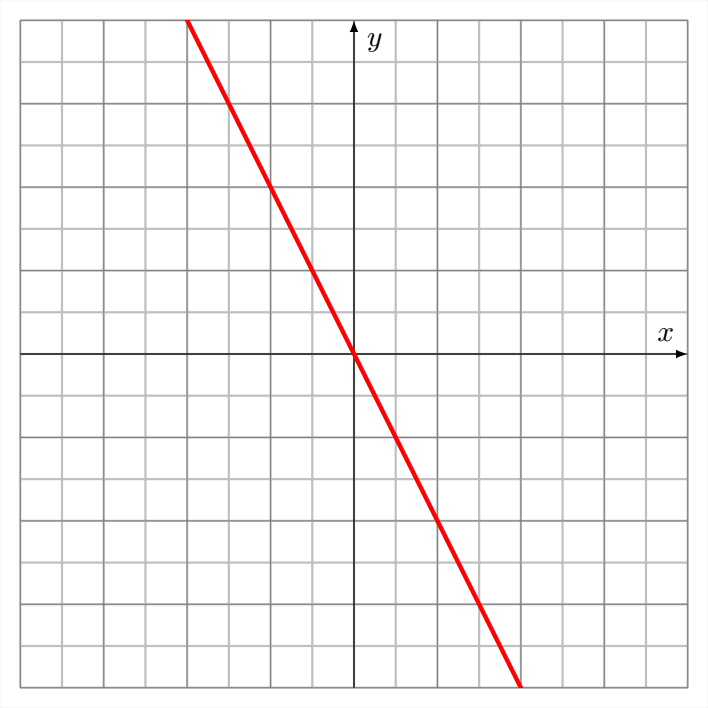
\includegraphics[width=140px]{../images/plano_cart_rect_-2x.png} \\[-0.5em]   \fillin[$-171$][1.5in]
                  \part 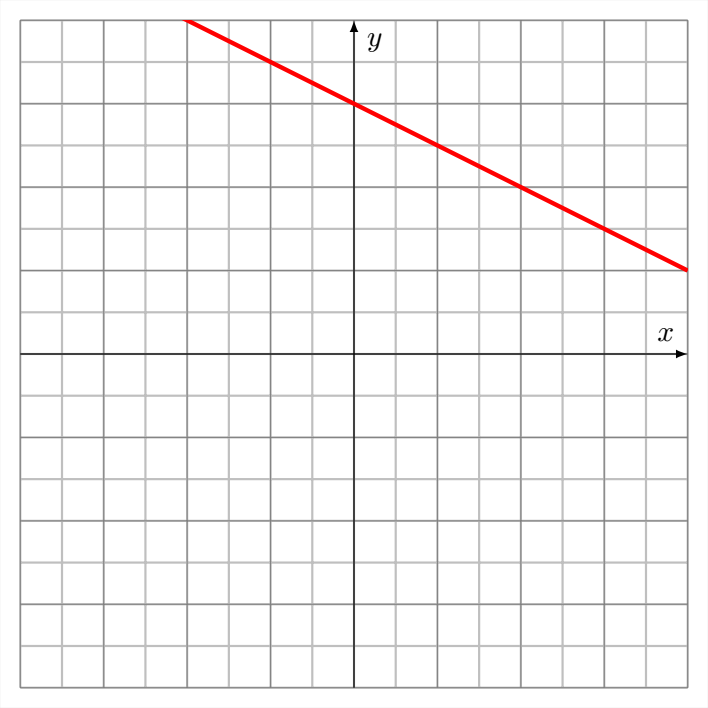
\includegraphics[width=140px]{../images/plano_cart_rect_-1|2x+4.png} \\[-0.5em]   \fillin[$-3$][1.5in]
                  \part 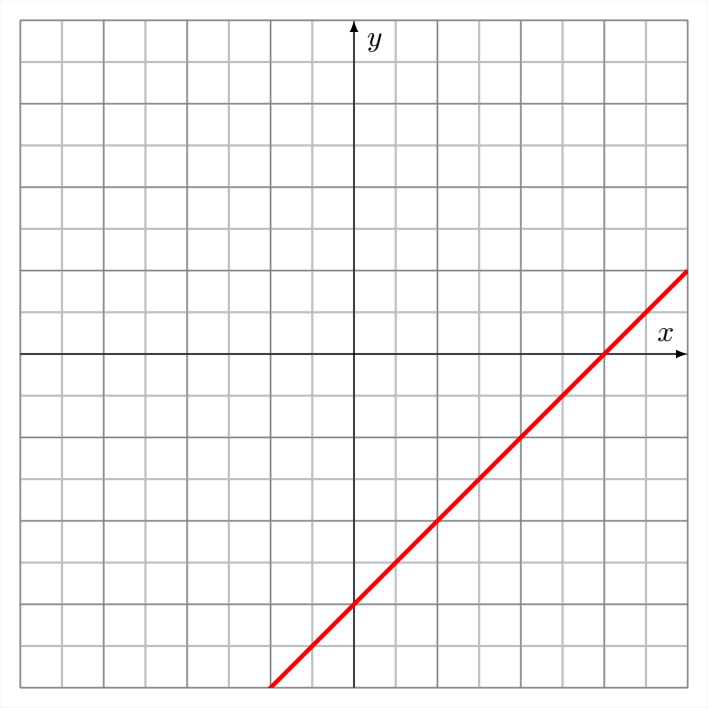
\includegraphics[width=140px]{../images/plano_cart_rect_x-6.png}  \\[-0.5em] \fillin[$-6$][1.5in]
                  \part 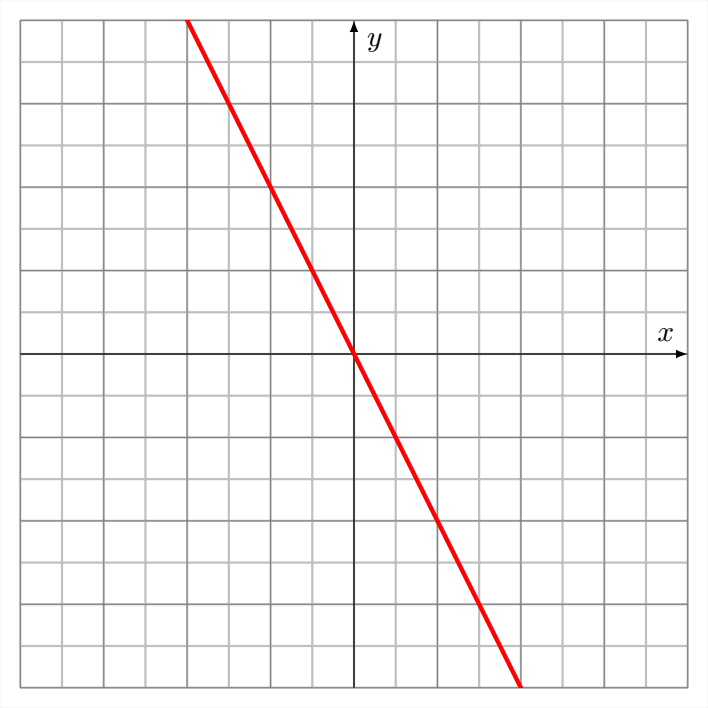
\includegraphics[width=140px]{../images/plano_cart_rect_-2x.png} \\[-0.5em]   \fillin[$-171$][1.5in]
            \end{parts}
      \end{multicols}

\end{questions}
\end{document}